%%%\scalebox{1.2}{ 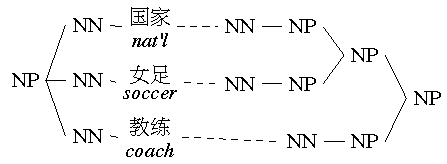
\includegraphics{figures/chinese-tree2} }

\begin{tikzpicture}
\tikzset{every tree node/.style={align=center}}
\Tree
[.NP 
  [.\extranode{NP}
    [.\extranode{NP} [.NN 国家\\national ] ]
    [.\extranode{NP} [.NN 女足\\soccer ] ] ]
  [.\extranode{NP} [.NN 教练\\coach ] ] ]
\end{tikzpicture}

\vspace{3mm}
(a) Parser output

\vspace{6mm}

\begin{tikzpicture}
\tikzset{every tree node/.style={align=center}}
\Tree
[.NP 
  [.NN 国家\\national ]
  [.NN 女足\\soccer ]
  [.NN 教练\\coach ] ]
\end{tikzpicture}

\vspace{3mm}
(b) Gold parse
\derivspace
\caption[Error analysis example: NP internal structure (Chinese).]{ \label{fig:np_internal} 
	\textbf{NP Internal Structure}: this should be a flat structure.
}
